\renewcommand\thechapter{\Roman{chapter}}
\chapter{Digital Forensics Investigation Case Study}
\newpage
\addcontentsline{toc}{section}{Introduction}
\section*{Introduction}
In this chapter, we are going to test some real case scenarios to show the usage and prove the efficiency of our platform. The scenarios are based on real attacks but any similarity in names is a mere coincidence. We will also try to link some of the investigation's outputs, as our project's purpose is not to automate the whole process and all the phases.\\
In order to simulate real scenarios, we prepared an attacker machine and a victim machine for two cases where we analyse the digital evidence after the extraction.


\section{Authentication and Dashboards}
In this section, we will present the authentication interface and the administration dashboard.\\
Figure IV.1 presents the first page of the platform, which is the authentication page. To access the platform's dashboards and functions, a user must enter his credentials in the login form.
\begin{figure}[H]
\centering
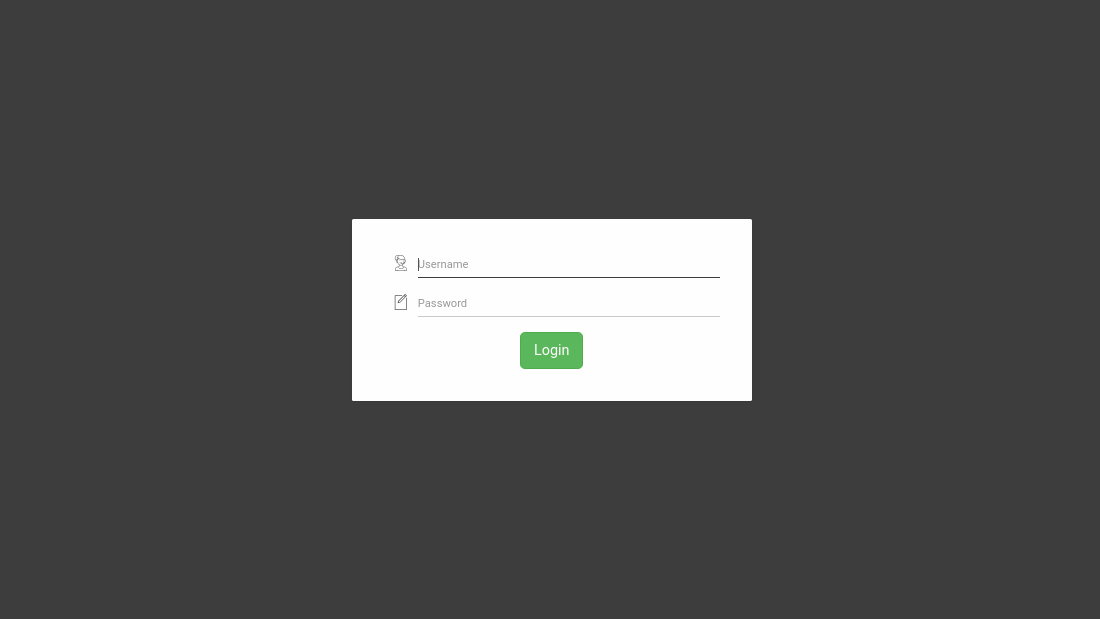
\includegraphics[width=0.9\columnwidth]{Figures/1.png}
\caption{The authentication page}
\end{figure}
Once the user is authenticated, drop-down menu appears on the top-right of the UI containing a logout link, and the administration dashboard's link, while the latter depends on whether the user is an administrator.\\
The first page we land on after a successful authentication, shown in Figure IV.2, allows a consultant to consult a case, remove it, or create a new one.
\begin{figure}[H]
\centering
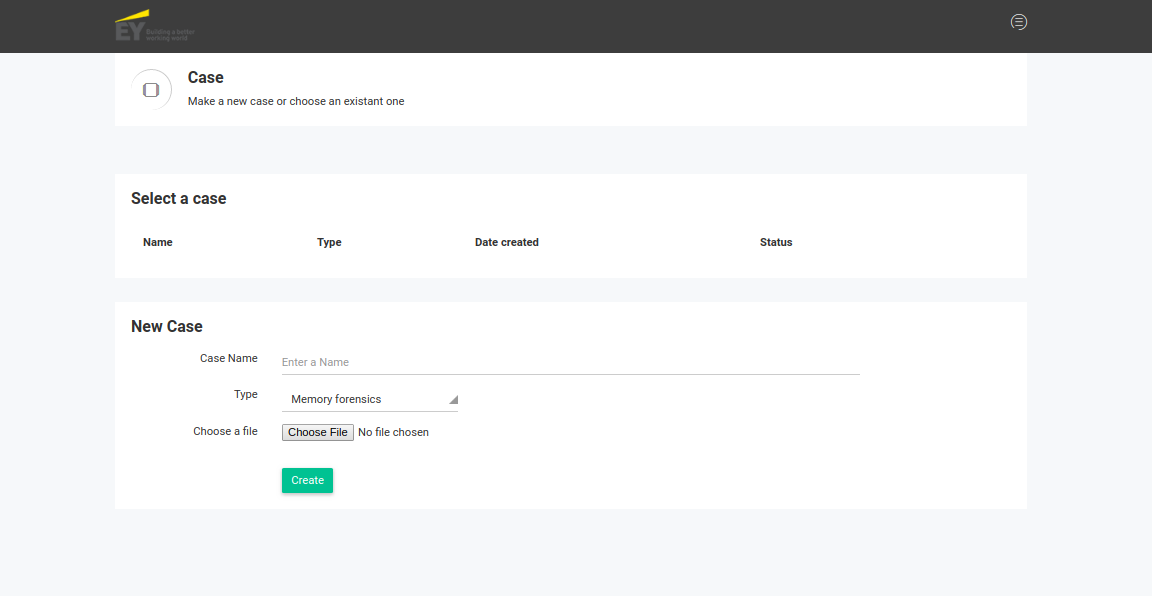
\includegraphics[width=0.9\columnwidth]{Figures/2.png}
\caption{Landing dashboard}
\end{figure}
Figure IV.3 presents the administration dashboard that can be accessed using the link provided in the menu for administrators. 
\begin{figure}[H]
\centering
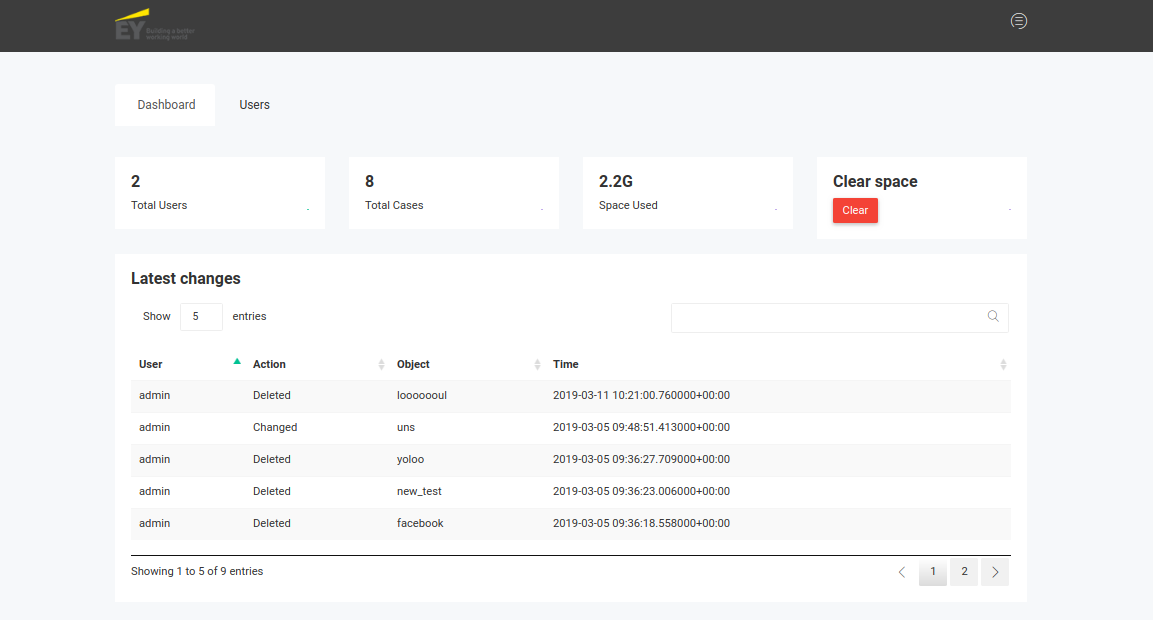
\includegraphics[width=0.9\columnwidth]{Figures/3.png}
\caption{The administration dashboard}
\end{figure}
On this page, the administrator can see some numbers that describe the platform and the database contents along with the latest changes made by users.\\
The administrator can also see the current users, add new ones, and edit the details of an existing user via the Users tab, which is presented in Figure IV.4.
\begin{figure}[H]
\centering
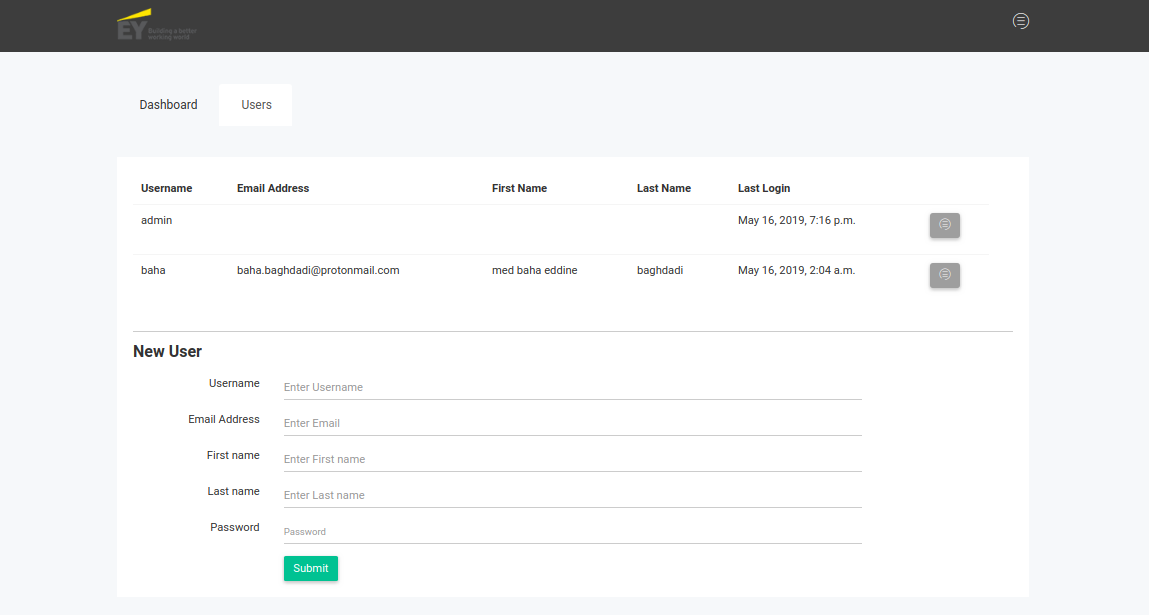
\includegraphics[width=0.9\columnwidth]{Figures/4.png}
\caption{The administration dashboard - Users tab}
\end{figure}

\section{Case Scenario 1: Potentially hacked teacher}
In this section, we will analyse a memory dump from a teacher's laptop that is suspected to have been hacked by a student, who eventually changed his exam score after gaining access.
\subsection{Creating the case}
The first step is extracting the memory dump using a tool like DumpIt\cite{dumpit}, or by simply retrieving the 'vmem' file created by Virtualbox of the victim's machine, in our case. Then, we start by filling out the corresponding form on the platform by supplying the case evidence file, case name, and case type, as is shown in Figure IV.5.
\begin{figure}[H]
\centering
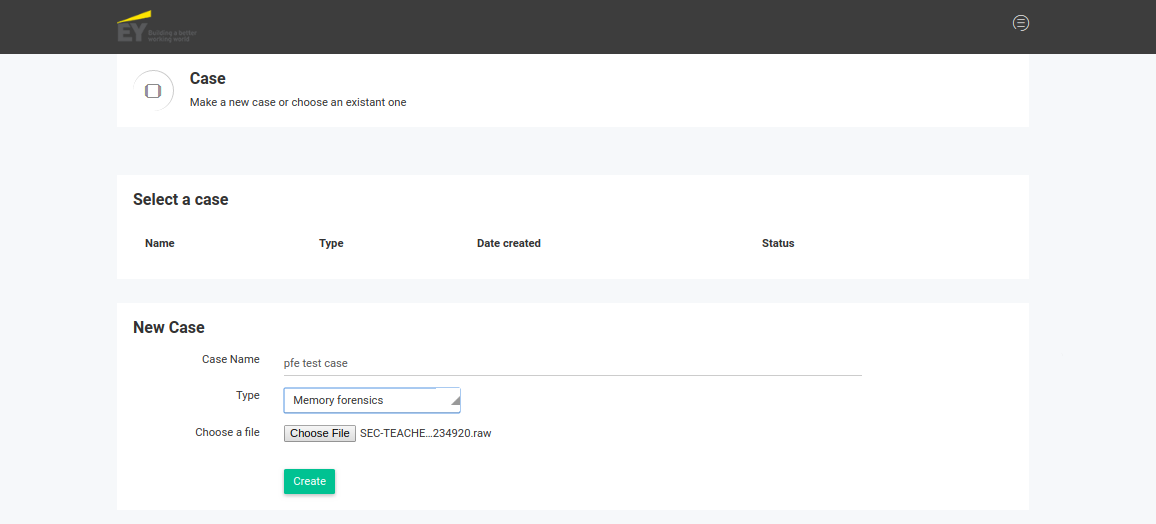
\includegraphics[width=0.9\columnwidth]{Figures/5.png}
\caption{Case creation}
\end{figure}
The evidence file is uploaded to the platform, the user is redirected to the same page, and we can see in Figure IV.6 that the green button labeled 'Pending' is disabled.
\begin{figure}[H]
\centering
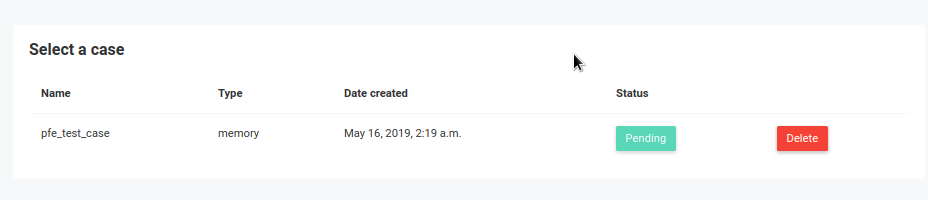
\includegraphics[width=0.9\columnwidth]{Figures/6.png}
\caption{Case file in analysis}
\end{figure}
The page keeps refreshing every 30 seconds to stay updated. After the analysis is done, the green button is enabled and labeled 'Ready', as seen in Figure IV.7
\begin{figure}[H]
\centering
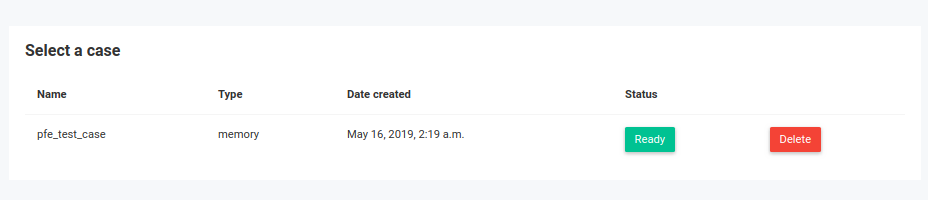
\includegraphics[width=0.9\columnwidth]{Figures/7.png}
\caption{Case analysis completed}
\end{figure}

\subsection{Reviewing the analysis}
The first page for a memory analysis contains general information about the case and the evidence file provided, and detected malicious behaviour like signature-based malware detected, keyloggers, and malicious reported IPs which we talked about in III.3.1.\\
Figure IV.8 presents an overview of how the memory analysis dashboard looks like.
\begin{figure}[H]
\centering
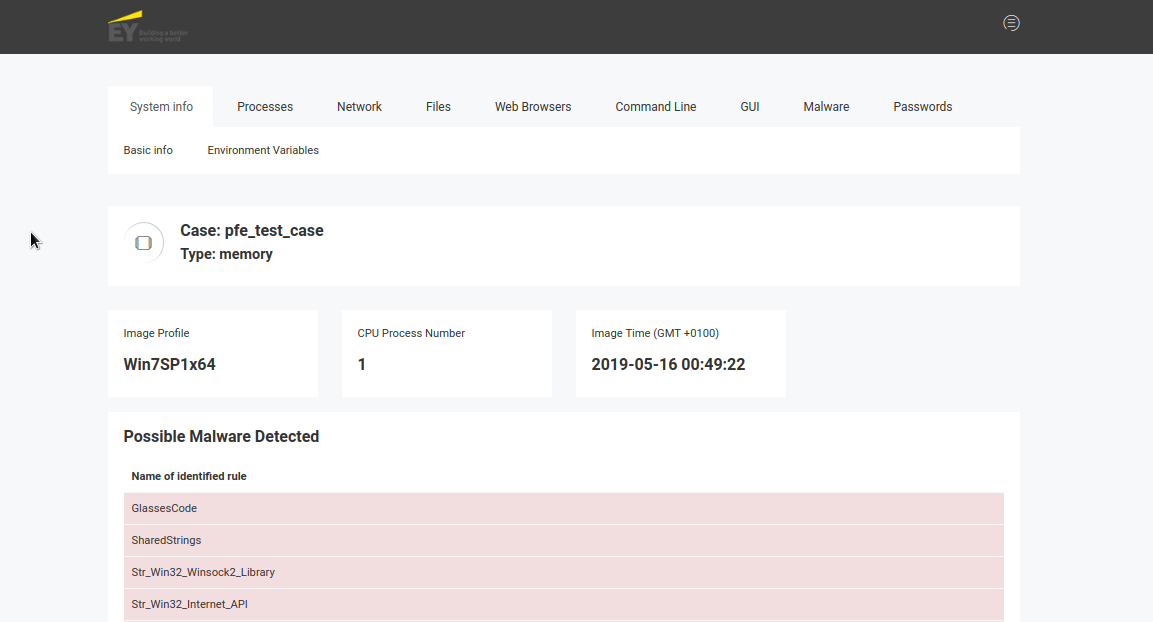
\includegraphics[width=0.9\columnwidth]{Figures/8.png}
\caption{Detected YARA rules in processes}
\end{figure}
Figure IV.9 shows the YARA rules detected in some of the processes.
\begin{figure}[H]
\centering
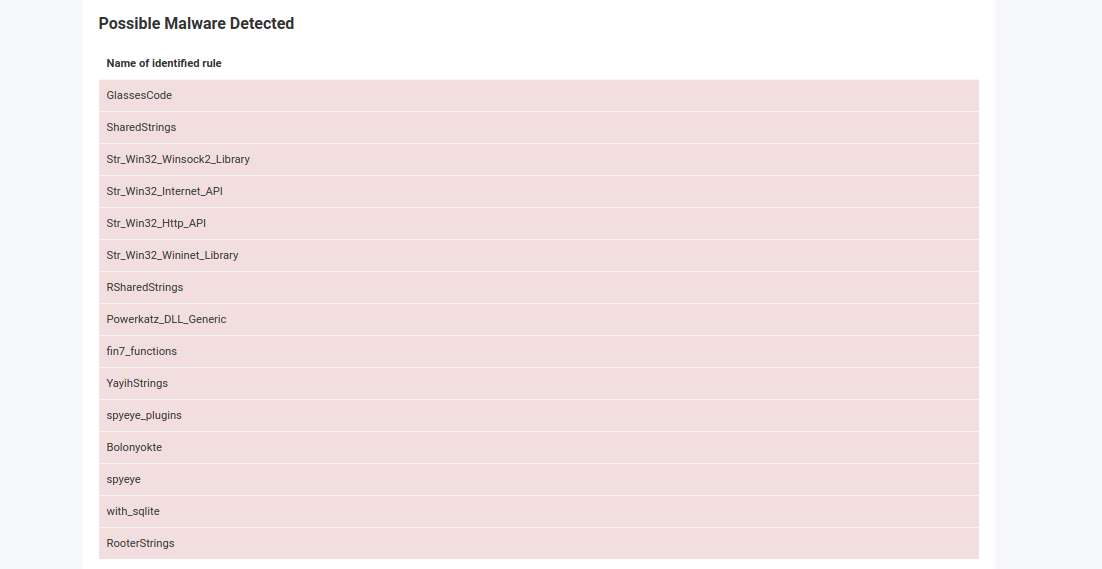
\includegraphics[width=0.9\columnwidth]{Figures/9.png}
\caption{Detected YARA rules in processes}
\end{figure}
Figure IV.10 shows the IP addresses that were reported as malicious and appeared in the computer's network connections.
\begin{figure}[H]
\centering
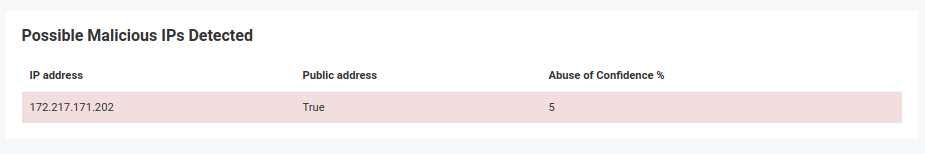
\includegraphics[width=0.9\columnwidth]{Figures/10.png}
\caption{Detected maliciously reported IP addresses}
\end{figure}
Figure IV.11 shows a detected keylogger process named 'rvlkl.exe', which goes back to a keylogger software named 'Revealer Keylogger'.
\begin{figure}[H]
\centering
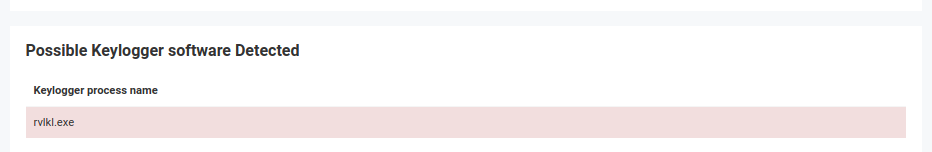
\includegraphics[width=0.9\columnwidth]{Figures/11.png}
\caption{Detected Keyloggers}
\end{figure}
\subsubsection{Malware analysis}
Following Figure IV.11, the detected rules based on YARA scan are 15 but that doesn't mean all the rules are of malware. For instance, the 'Str\_Win32\_Internet\_API' rule means that a process is calling the Windows Inet API, which may be sending a reverse shell but no necessarily. The 'fin7\_functions' though, is relevant to a malware attack previously used by a group of hackers called FIN7 that downloads and executes shellcode, which looks interesting enough to look for details in the full YARA analysis, like shown in Figure IV.12.
\begin{figure}[H]
\centering
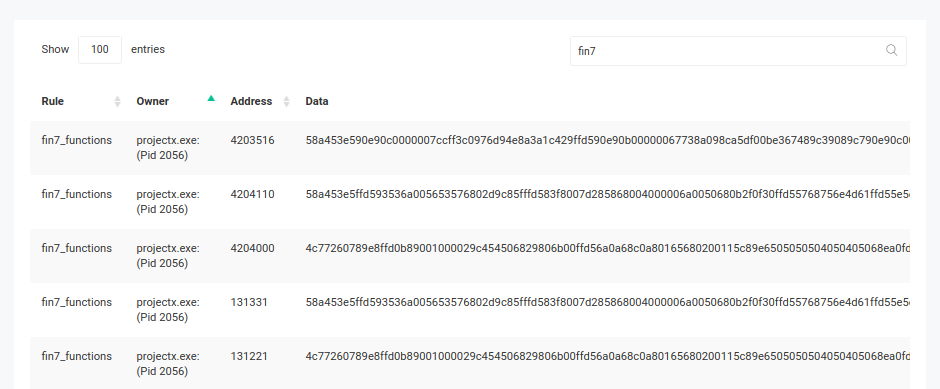
\includegraphics[width=0.9\columnwidth]{Figures/12.png}
\caption{YARA scan filtered to 'fin7'}
\end{figure}
We can conclude that it points to a process named 'projectx.exe'. Figure IV.13 shows the output we get from YARA scan if we filter on the previously named process, which by the look of it, is using the internet. So, next step is to look at the network connections following this process and scan the process executable.
\begin{figure}[H]
\centering
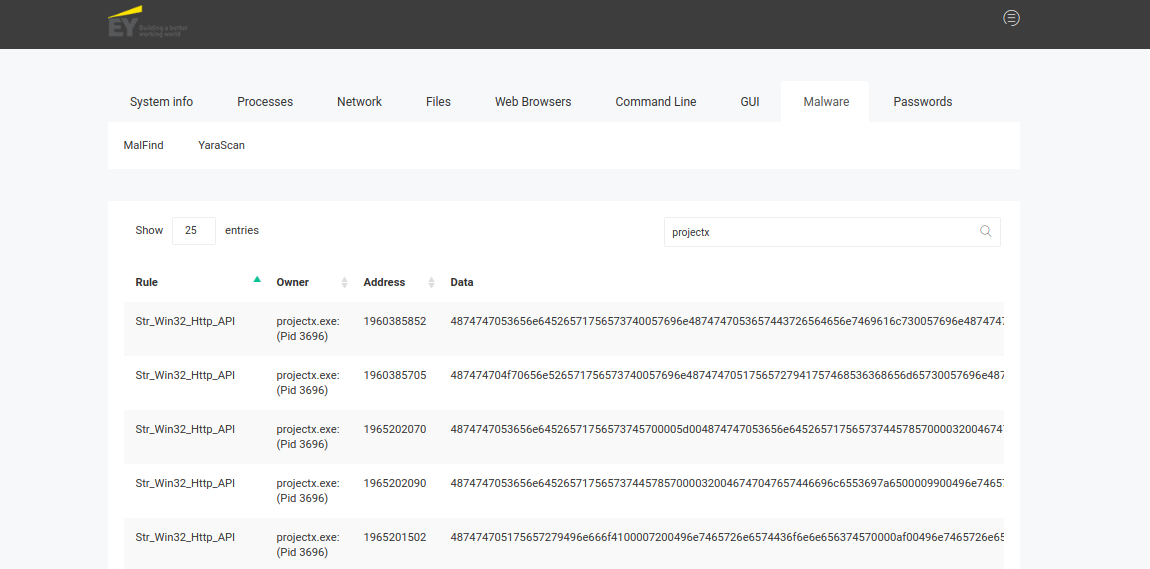
\includegraphics[width=0.9\columnwidth]{Figures/13.png}
\caption{YARA scan filtered to 'projectx'}
\end{figure}
\subsubsection{Network connections}
The network connections established on the victim's computer looked normal, but as we suspected previously, Figure IV.14 shows that the process 'projectx.exe' was sending a connection to another IP on the same network and using port 4444.
\begin{figure}[H]
\centering
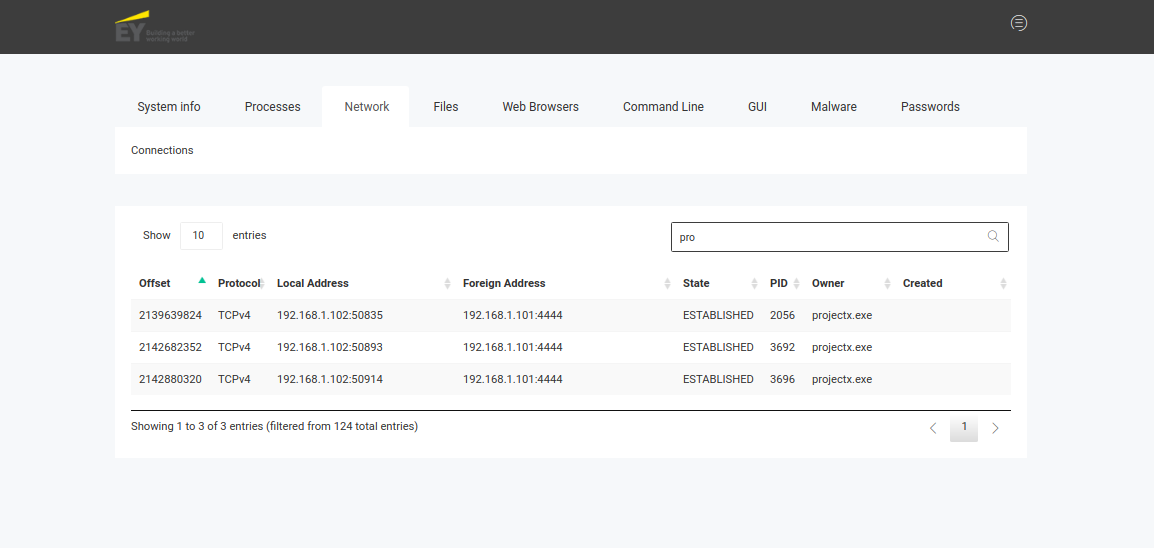
\includegraphics[width=0.9\columnwidth]{Figures/14.png}
\caption{Network connections filtered to 'projectx'}
\end{figure}
\subsubsection{Process analysis}
The process was found to be using the internet to send data, potentially a reverse shell, to another computer. As presented in Figure IV.15, for more analysis we can dump the process executable using the Dump button corresponding to the process, and reverse engineer it and submit it for analysis on VirusTotal.
\begin{figure}[H]
\centering
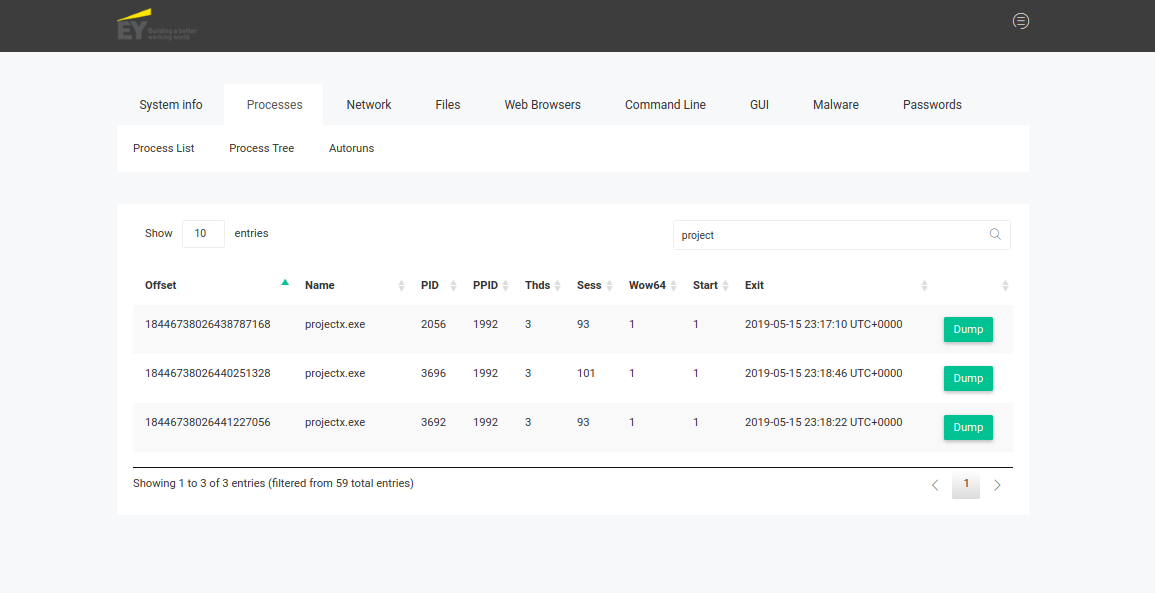
\includegraphics[width=0.9\columnwidth]{Figures/15.png}
\caption{Process details}
\end{figure}
Figure IV.16 shows the analysis report from VirusTotal that detected the executable as malicious.
\begin{figure}[H]
\centering
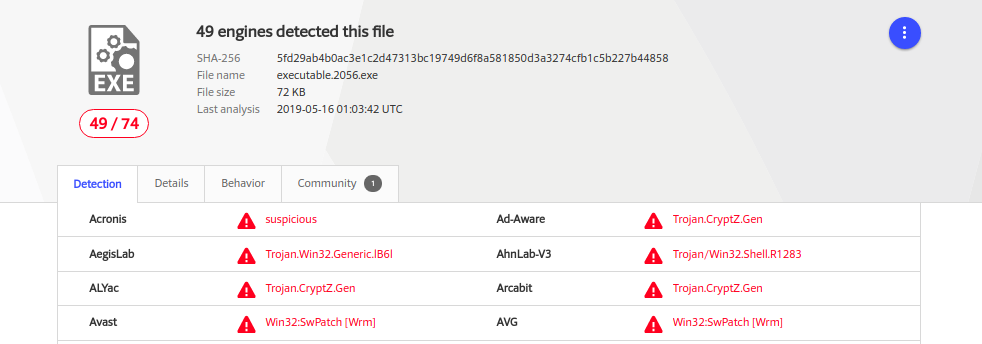
\includegraphics[width=0.9\columnwidth]{Figures/16.png}
\caption{VirusTotal analysis report}
\end{figure}
We now need to know how the file was executed. It is possible that the teacher ran the file without detecting it was malicious, or it was executed automatically from a malicious website script, or another way. We can see the background command used to launch the file using the module we described in III.3.1.8 as follows in Figure IV.17.
\begin{figure}[H]
\centering
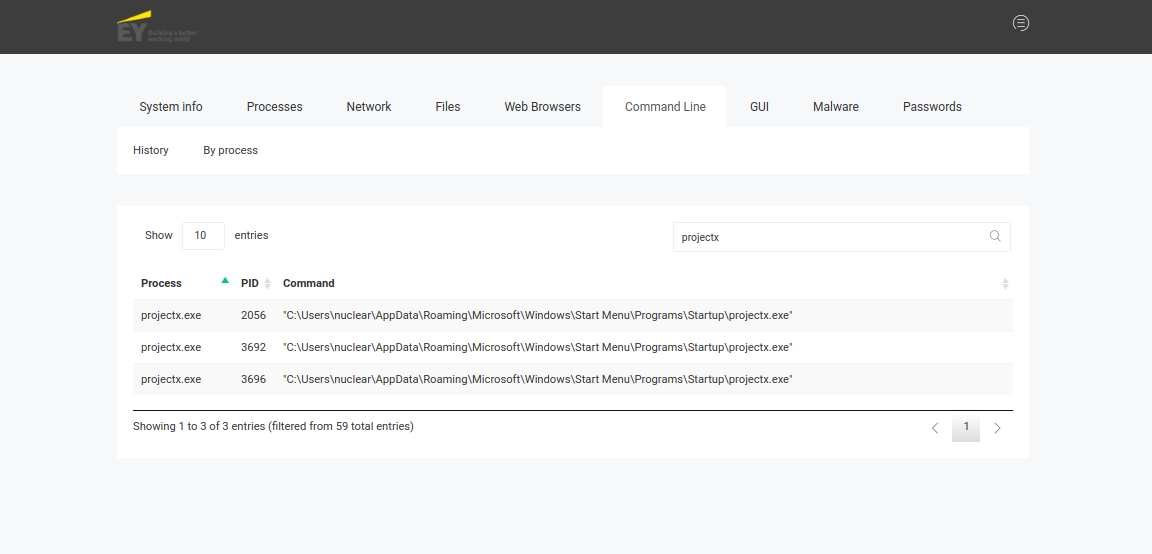
\includegraphics[width=0.9\columnwidth]{Figures/17.png}
\caption{Command Line analysis for projectx.exe}
\end{figure}
Following the link from where the file was launched, it is to be believed that the malware was planted another way before and is now launched every time the teacher starts his computer.
\subsubsection{Tracking the victim's activity}
To know how the teacher's computer was infected we must look at the browser history, screenshots, and files that the he accessed.\\
The chrome history in Figure IV.18 is a raw list of links accessed by the user on Google Chrome. The user accessed his email, his Google drive and a website called projectx and downloading some files which are proven to be malicious.
\begin{figure}[H]
\centering
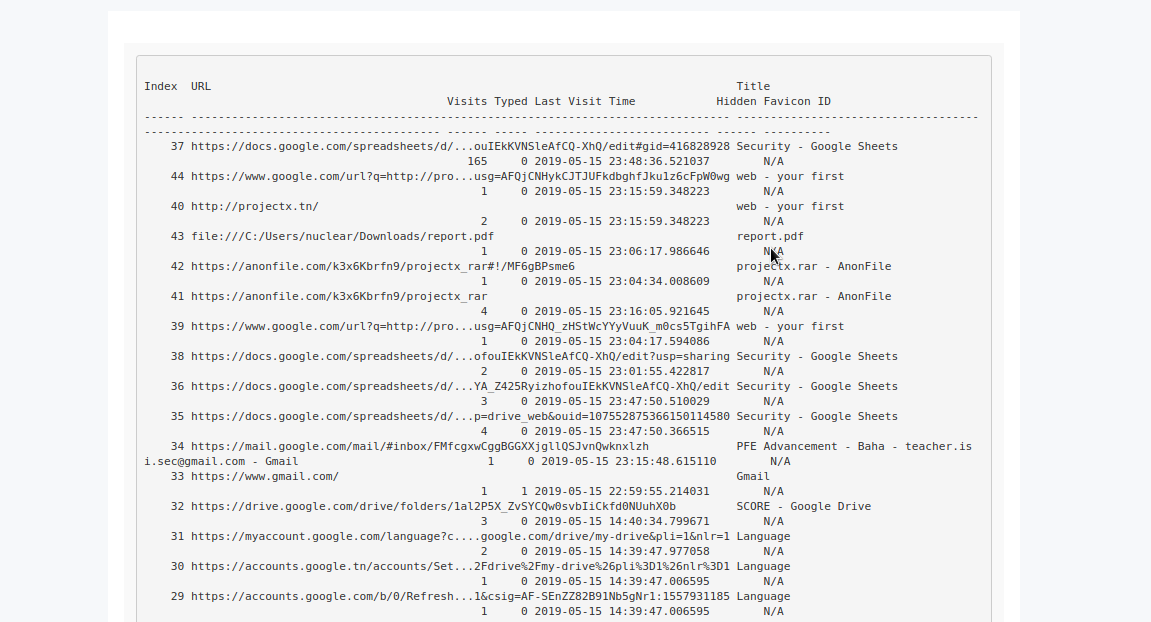
\includegraphics[width=0.9\columnwidth]{Figures/18.png}
\caption{Chrome history extracted}
\end{figure}
Looking for file that the user accessed will be available to find since it should still be in the memory. We can see a very long list of files and possibly filter and extract some of them in the Files tab, as shown in Figure IV.19.
\begin{figure}[H]
\centering
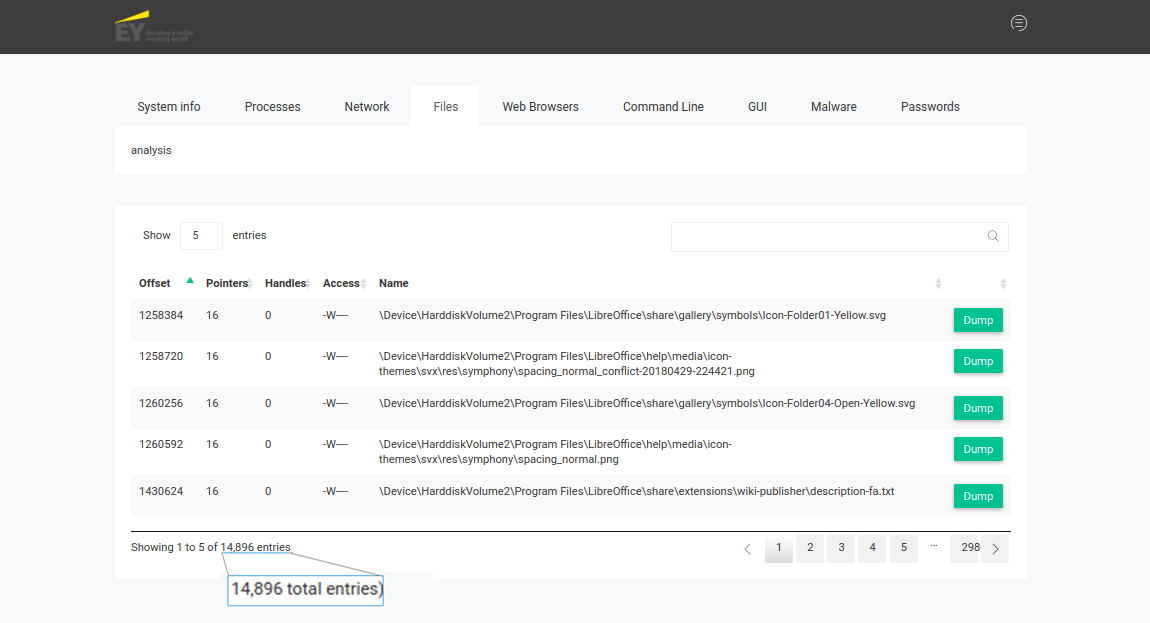
\includegraphics[width=0.9\columnwidth]{Figures/19.png}
\caption{File scan output}
\end{figure}
As displayed in Figure IV.20, filtering on the Documents, Desktop, and other home folders did show an interesting file. This file is a screenshot, presented in Figure IV.21, was taken by the teacher upon receiving an email.
\begin{figure}[H]
\centering
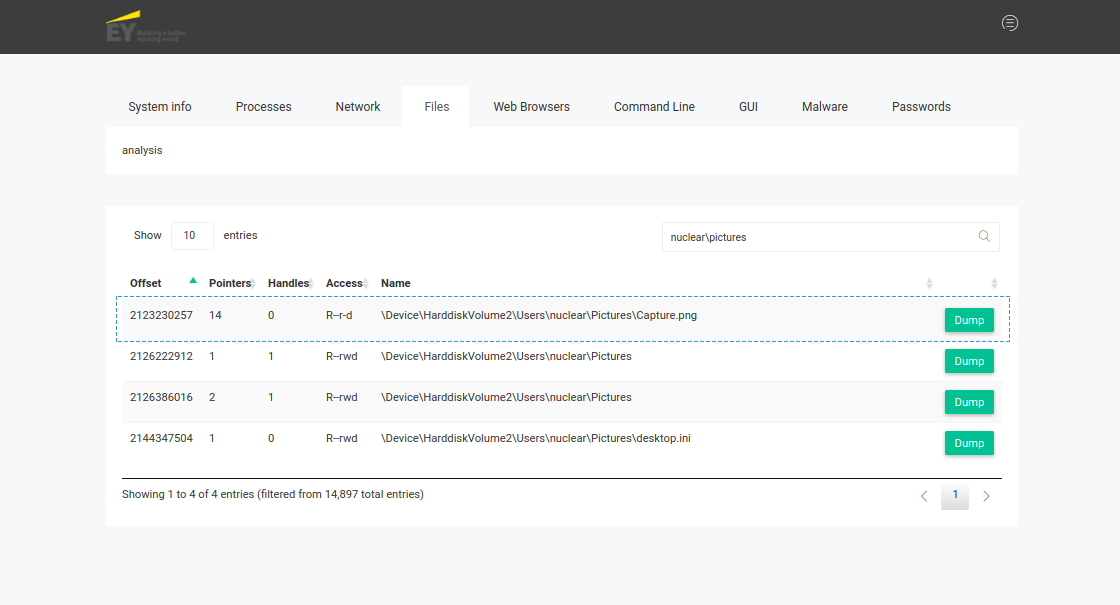
\includegraphics[width=0.9\columnwidth]{Figures/20.png}
\caption{Filtering files to Pictures folder}
\end{figure}
Following the screenshot in Figure IV.21, we are sure that the email sent by the student was part of the sequence that led the teacher to access the Projectx website that infected the teacher's computer.
\begin{figure}[H]
\centering
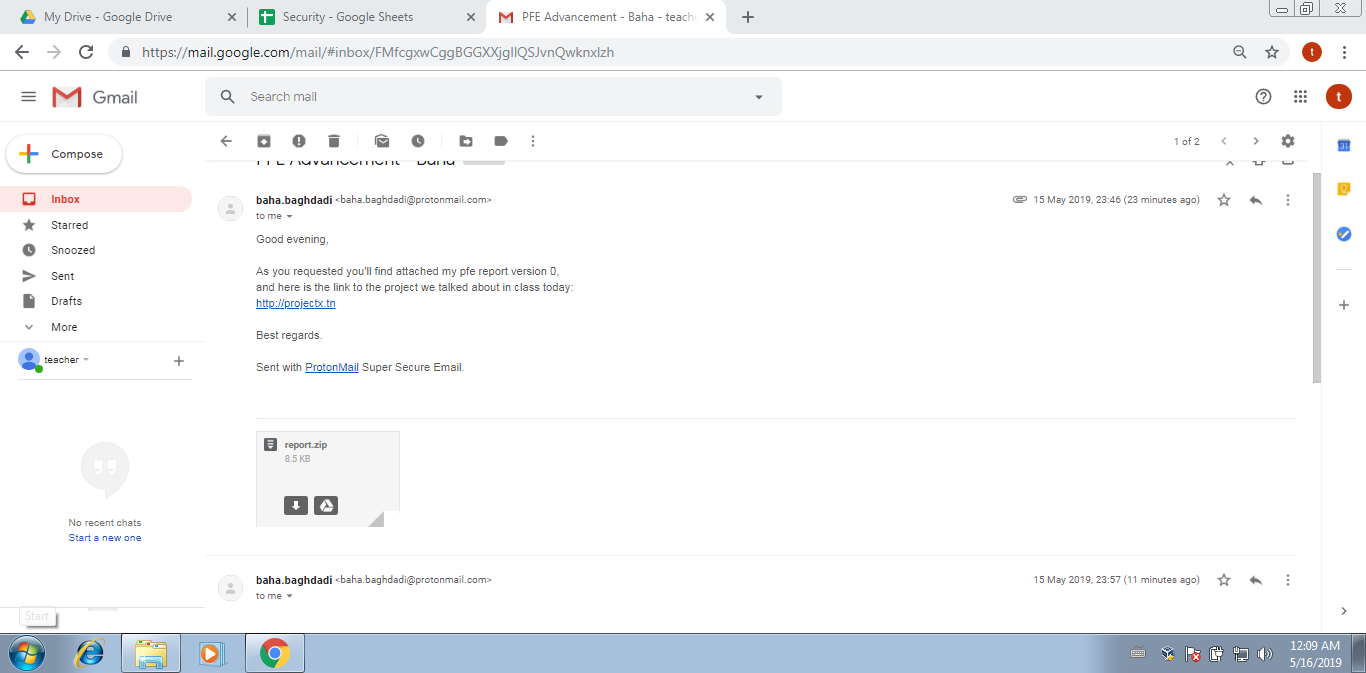
\includegraphics[width=0.9\columnwidth]{Figures/21.png}
\caption{Dumped screenshot file}
\end{figure}
Also the keylogger that we detected earlier should be saving to a file on the system which can look for by filtering the files detected in the memory to 'rvlkl'. As Figure IV.22 reveals, we found and can dump the log file (.rvl extension) of the keylogger.
\begin{figure}[H]
\centering
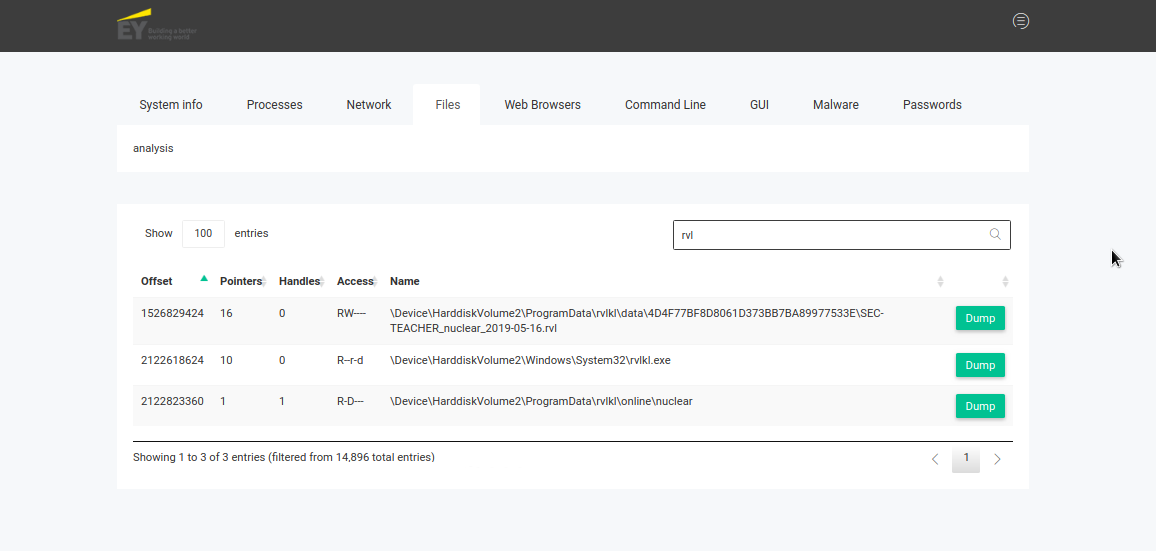
\includegraphics[width=0.9\columnwidth]{Figures/22.png}
\caption{Keylogger log file}
\end{figure}

\subsection{Case outlooks}
A point we did not focus on, was the malicious IP we've seen on Figure IV.10. Based on that IP and the other detected YARA rules, we can nearly confirm that the keylogger and possibly the virus in question, were planted after another attack associated with that address and linking to an earlier malware infection. We answered a lot of questions using only the memory dump. Some of the points we found are:
\begin{itemize}
    \item Where the virus came from.
    \item The type of the virus.
    \item How the virus got executed.
    \item Attacker's local IP address.
    \item Are there any other malware planted.
\end{itemize}
The rest of the case is not memory analysis, but rather linking the collected artifacts and following the allegation of the teacher which stated that a student's note was altered.\\
We will not continue breaking down the case, but, the teacher's allegation is true since the scores were on the link he visited (see Figure IV.18) and the log for the Drive shows an anonymous edit to the file at the time of the attack.\\
A breakdown of the network traffic can also showcase the commands ran by the hacker remotely through port 4444.\\

\section{Case Scenario 2: Malware infected computer}
In this section, we will analyse both a memory dump and a network traffic from a malware infected computer that was detected to be connected to suspecious IP addresses.
\subsection{Creating the case}
The first step is extracting the memory dump using a tool like DumpIt, and saving the network traffic as a pcap file. Then, we start by filling out the corresponding form on the platform by supplying the case evidence file, case name, and case type. Figure IV.23 shows the interface after both analysis are ready.
\begin{figure}[H]
\centering
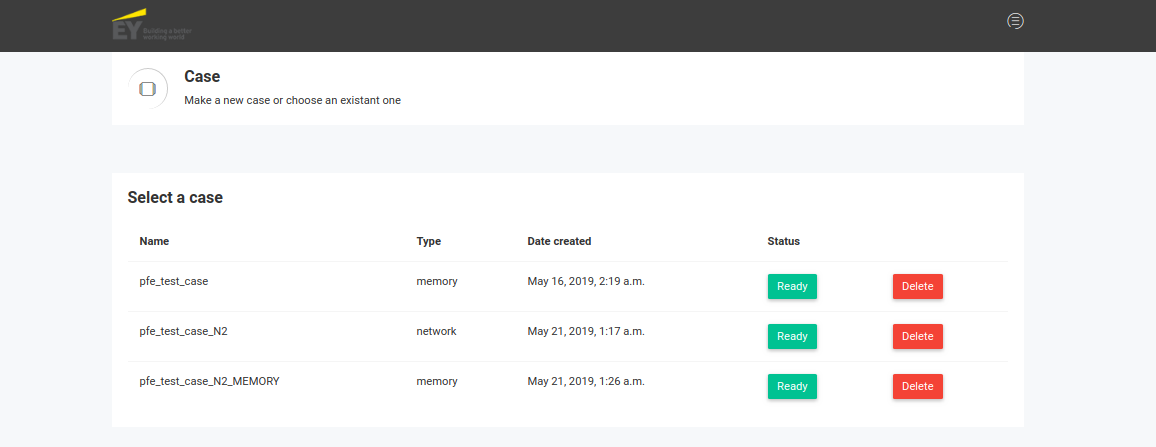
\includegraphics[width=0.9\columnwidth]{Figures/23.png}
\caption{Case 2 creation}
\end{figure}
\subsection{Reviewing the memory analysis}
Starting with the memory dump, the first page shows detected malicious traces. The first thing we focus on is the malware signatures detected, as presented in Figure IV.24. We can see Mirage\_APT and xtreme\_rat YARA rules, which indicate that there might be an APT present on the system.
\begin{figure}[H]
\centering
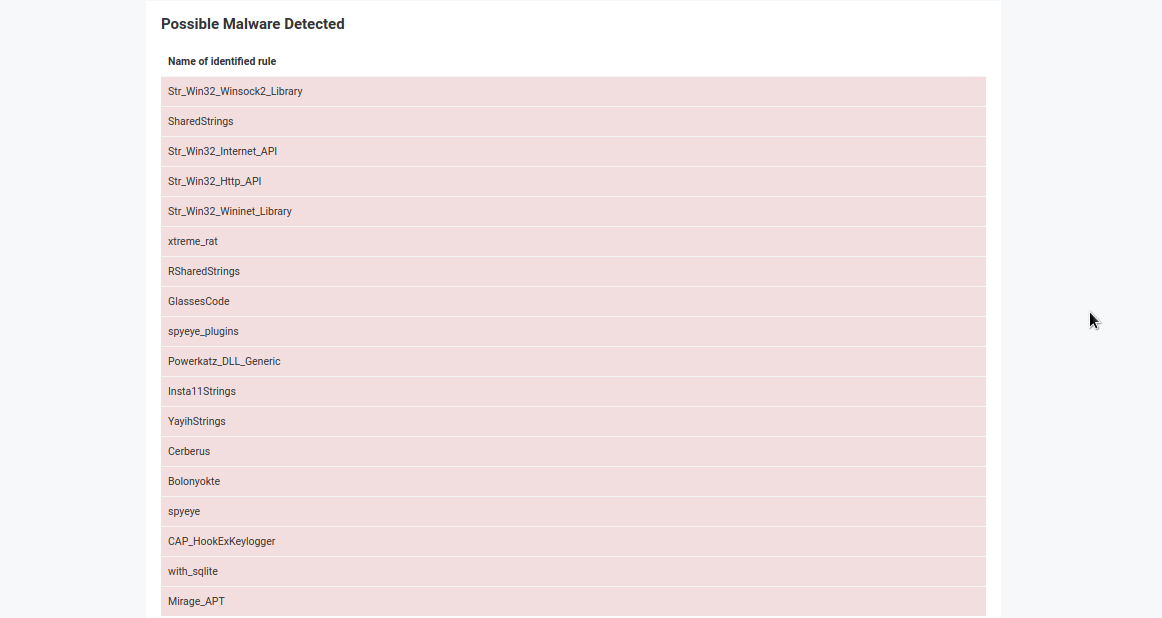
\includegraphics[width=0.9\columnwidth]{Figures/24.png}
\caption{Detected malware YARA signatures}
\end{figure}
Figure IV.25 presents the malicious IP addresses detected.
\begin{figure}[H]
\centering
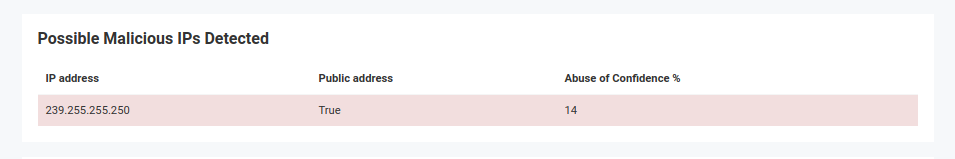
\includegraphics[width=0.9\columnwidth]{Figures/25.png}
\caption{Detected malicious IP}
\end{figure}
\subsubsection{Network connections}
We can then look for the connections made by the computer to the previously detected IP address in the network tab. As seen in Figure IV.26, the connection has been closed and was the computer was connecting to a web server on port 80.
\begin{figure}[H]
\centering
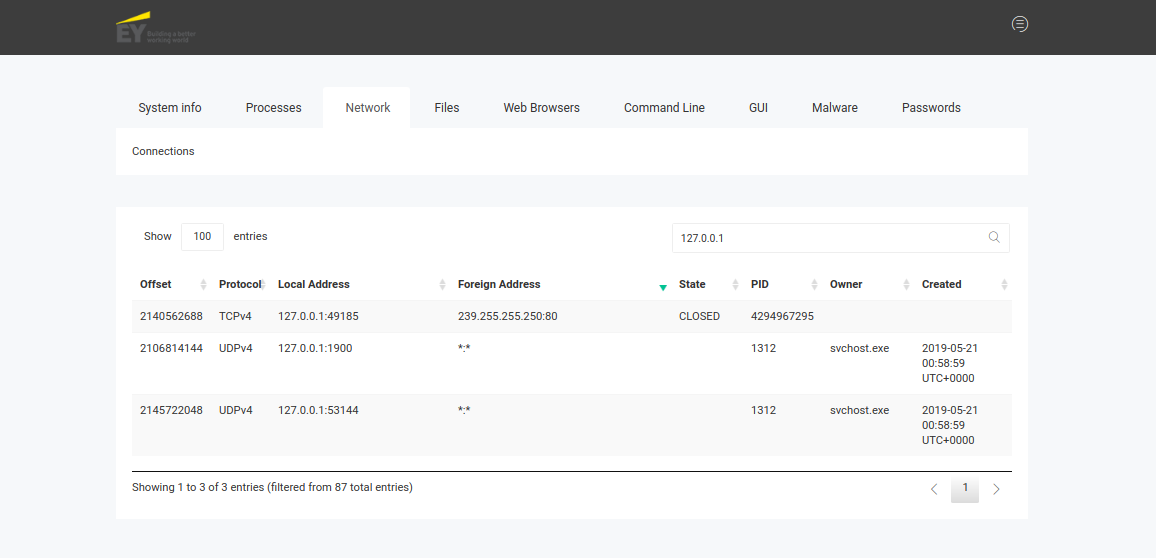
\includegraphics[width=0.9\columnwidth]{Figures/26.png}
\caption{Network connection to malicious IP}
\end{figure}
Figure IV.27 clears that by checking the Google Chrome history, we can see the domain name that should correspond to that IP as it was the only connection made through this browser.
\begin{figure}[H]
\centering
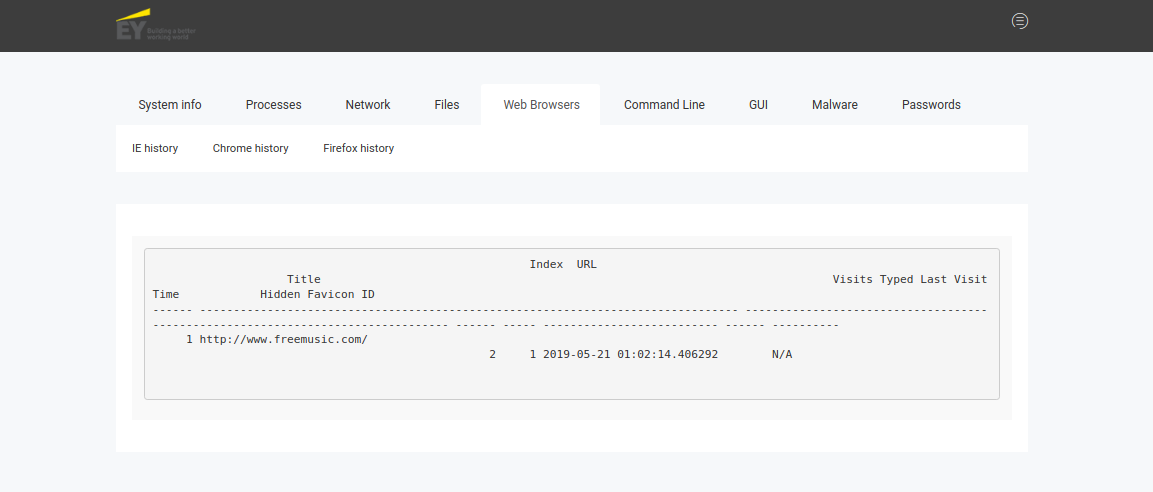
\includegraphics[width=0.9\columnwidth]{Figures/27.png}
\caption{Chrome history}
\end{figure}
\subsubsection{Malware Detection}
As seen before, we need to check the detected YARA rules in process thoroughly to make sure they aren't all false-positives. As presented in Figure IV.28, Filtering the output to 'Mirage\_APT' bring out the Google Chrome process, linking our first idea that the domain in Chrome history is the malware initiator.
\begin{figure}[H]
\centering
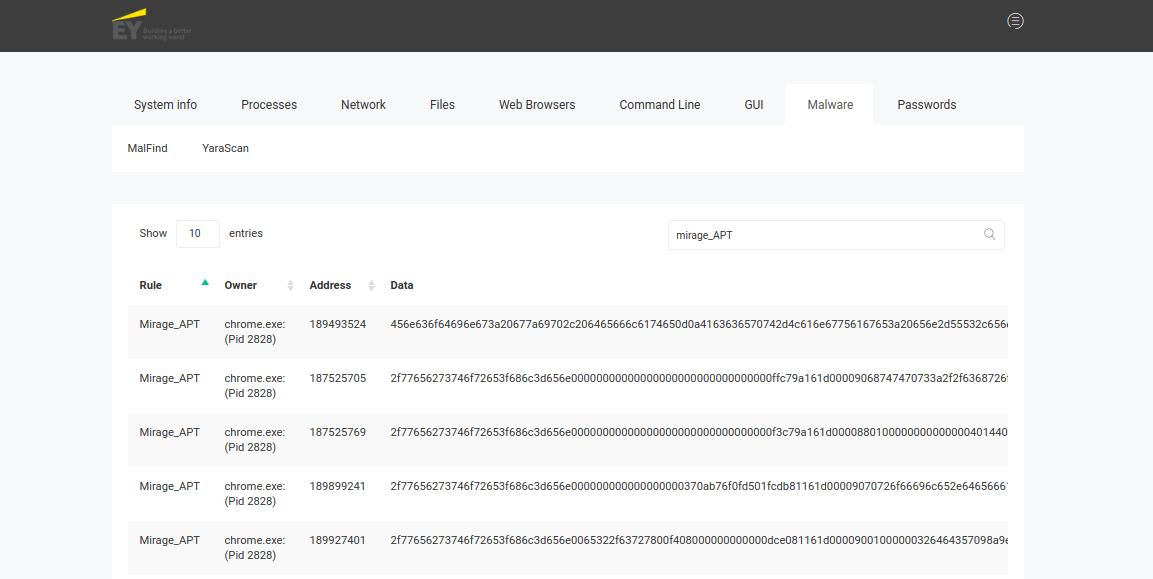
\includegraphics[width=0.9\columnwidth]{Figures/28.png}
\caption{YARA scan Mirage APT filtered}
\end{figure}
The memory analysis gives us some idea about the malware infection, but since it was done through the internet, we can't get the files requested by the browsers like javascript and flash scripts. The network traffic analysis is therefore needed.
\subsection{Reviewing the network analysis}
It is important to analyse the network traffic to explain what happened between the computer and the suspected malicious server. In this section, we need to know what happened in that conversation.
Figure IV.29 presents the landing page of the network analysis. This page provides general information about the case and the evidence file provided.
\begin{figure}[H]
\centering
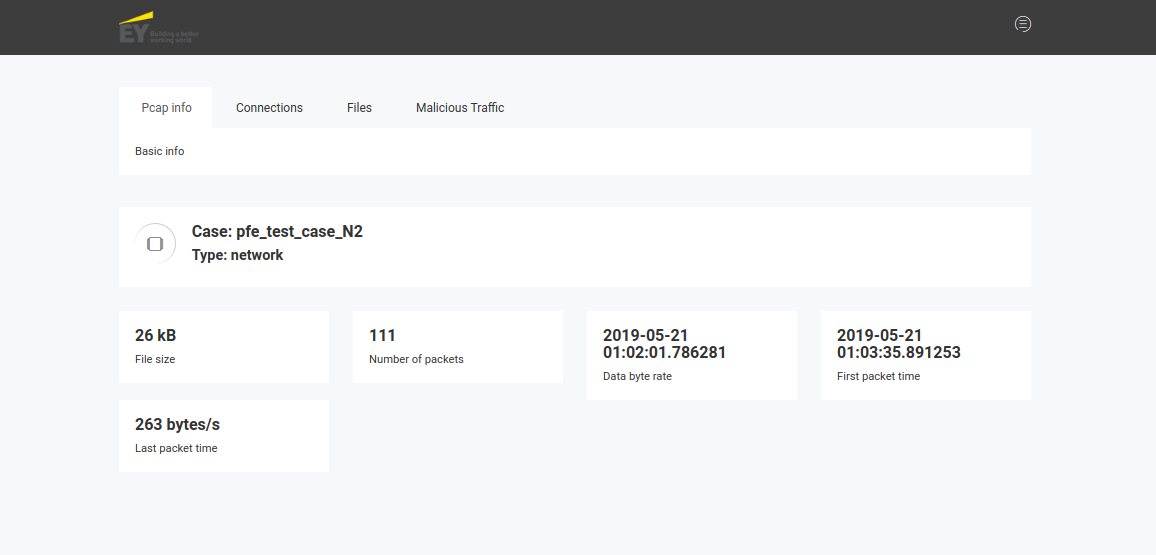
\includegraphics[width=0.9\columnwidth]{Figures/29.png}
\caption{Network analysis landing page}
\end{figure}
The connection made by the computer was to an HTTP server, so heading to the malicious traffic tab should present us with a summary and detailed information about the HTTP conversations detected, and an analysis of the transferred objects. Figure IV.30 presents the summary output of this tab. As we can see, the only conversation available is the one made with the domain we extracted from the memory dump: 'www.freemusic.com' but the IP isn't the one we found as malicious. This means that the web server and the command & control server of the attacker are separate.
\begin{figure}[H]
\centering
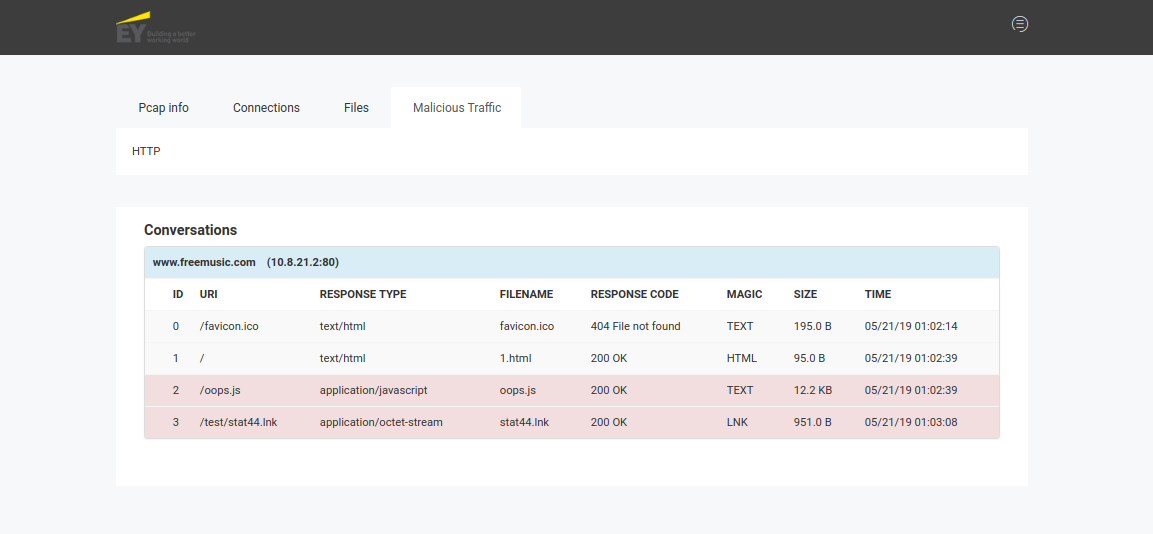
\includegraphics[width=0.9\columnwidth]{Figures/30.png}
\caption{Malicious HTTP traffic scan summary}
\end{figure}
The lines in red point to a suspicious file. Starting with the first file, which is a javascript script, Figure IV.31 represents the details on the object, after clicking on it. We see the request, response, and a portion of the file's content. We also have a download button to extract the file from the traffic, and the hash of the file which links to it's analysis on VirusTotal.
\begin{figure}[H]
\centering
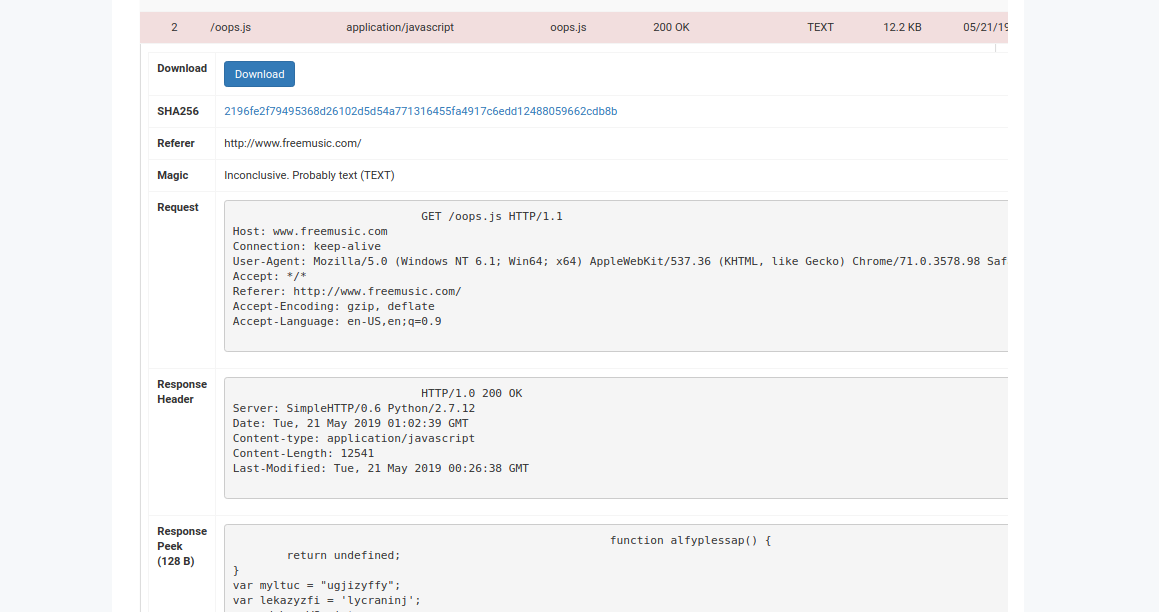
\includegraphics[width=0.9\columnwidth]{Figures/31.png}
\caption{Suspicious javascript object details}
\end{figure}
When clicking on the file's hash, we are redirected to the analysis report generated on VirusTotal of this file, which is seen in Figure IV.32. The script does appear to be a proven trojan script, which might have started the infection.
\begin{figure}[H]
\centering
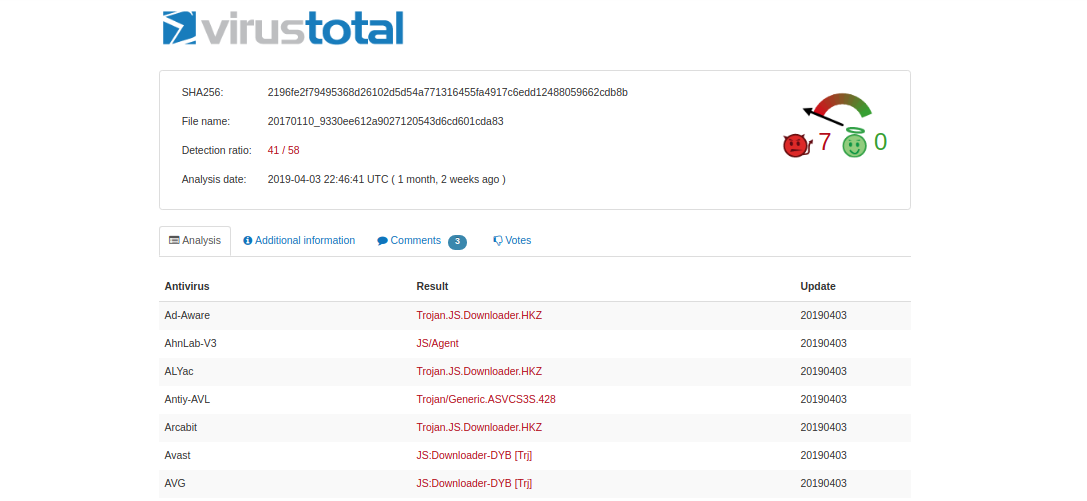
\includegraphics[width=0.9\columnwidth]{Figures/32.png}
\caption{JavaScript file analysis on VirusTotal}
\end{figure}
The second file is a windows shortcut file that was apparently downloaded on the system with the previous javascript code. This file can execute a command when run. Figure IV.33 shows the details on the object, after clicking on it.
\begin{figure}[H]
\centering
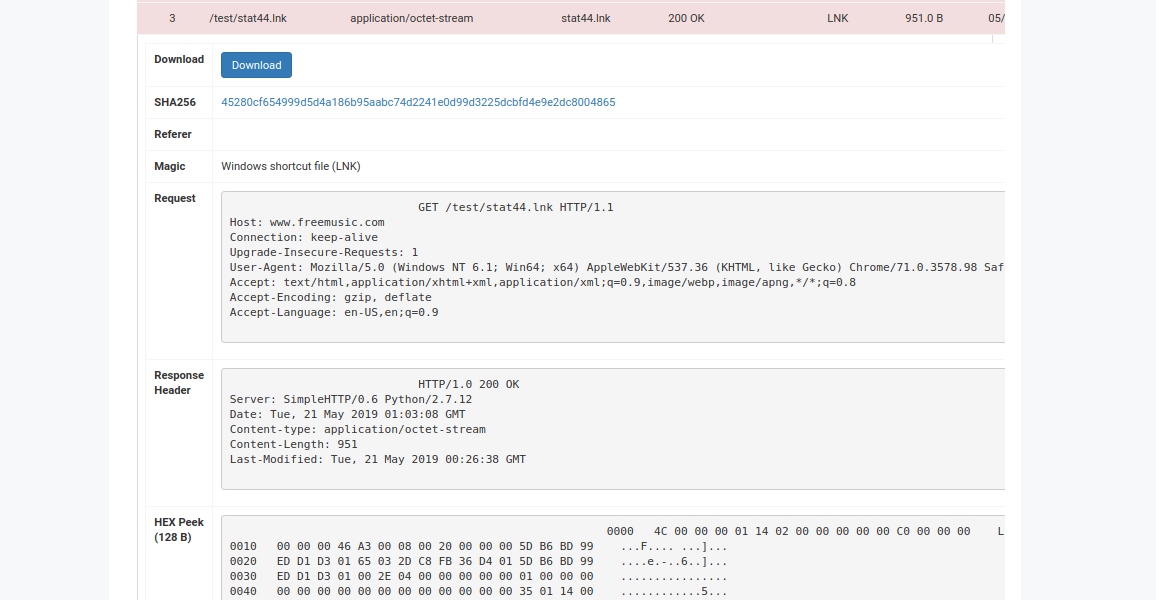
\includegraphics[width=0.9\columnwidth]{Figures/33.png}
\caption{Suspicious lnk object details}
\end{figure}
Clicking on the hash of the file brings us the report from VirusTotal, included in Figure IV.34. The file is proven to be an autorun powershell malicious script and must be the file that executes the APT on the system.
\begin{figure}[H]
\centering
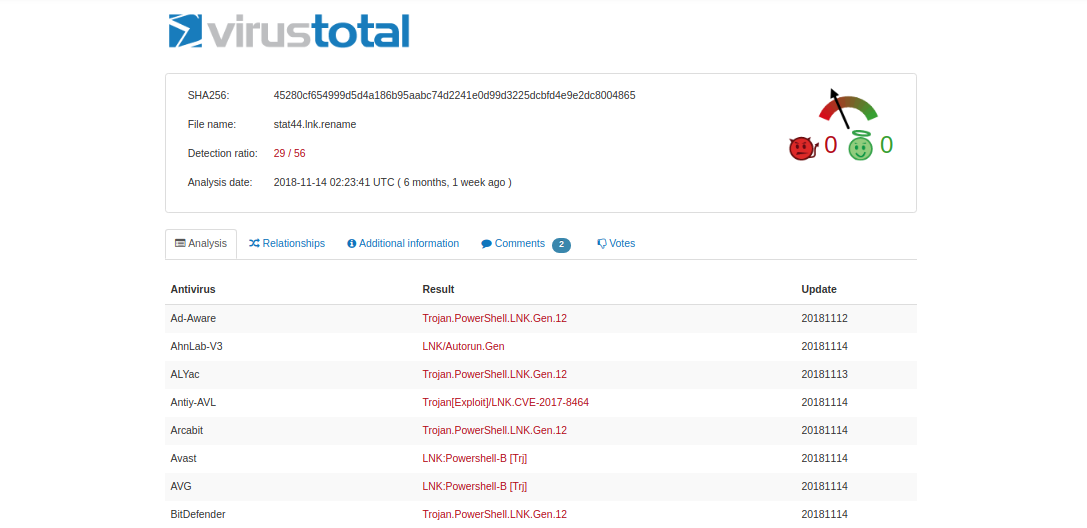
\includegraphics[width=0.9\columnwidth]{Figures/34.png}
\caption{Lnk file analysis on VirusTotal}
\end{figure}
\subsection{Case outlooks}
In this case, we analysed the memory dump and network traffic together for better understanding of what we faced. The Link between both analysis is kept manual because of the complications that could have happened and the high number of false-positive that could appear, as we saw when we expected the web server to be the attacker's command \& control server. Some of the answers we got and help us build our report on this case are:
\begin{itemize}
    \item The infection process of the malware into the computer.
    \item The nature of the malware and it's code.
    \item Domain and IP of the attacker's web server.
    \item IP of the attacker's C\&C server.
\end{itemize}
After the analysis we can conclude that the suspicious domain executes a script and redirects you to other pages like ads that could install and execute shortcut files so fast that it would complete it's mission when you close it.
\addcontentsline{toc}{section}{Conclusion}
\section*{Conclusion}
Throughout this chapter, we presented the platform's user interface and how it serves in the analysis of digital evidence. We tested the application's modules' capabilities by performing a nearly full digital forensics investigation to showcase it's usage in the real world.